\subsubsection{Arten von Suchmaschinen}

\begin{itemize}
  \item \textbf{Universalsuchmaschinen} $\rightarrow$ durchsuchen das Web für Durchschnittsnutzer
  \item \textbf{Spezialsuchmaschinen} $\rightarrow$ thematische Beschränkung für zielgenaue Recherche
  \item \textbf{Metasuchmaschinen} $\rightarrow$ die besten Ergebnisse mehrerer Suchmaschinen
  \item \textbf{Suchdienste} $\rightarrow$ Web-Verzeichnisse, Social Bookmarking, Frage-Antwort-Dienste
\end{itemize}

\clearpage
\subsubsection{Aufbau von Suchmaschinen}

\begin{figure}[ht]
\begin{center}
  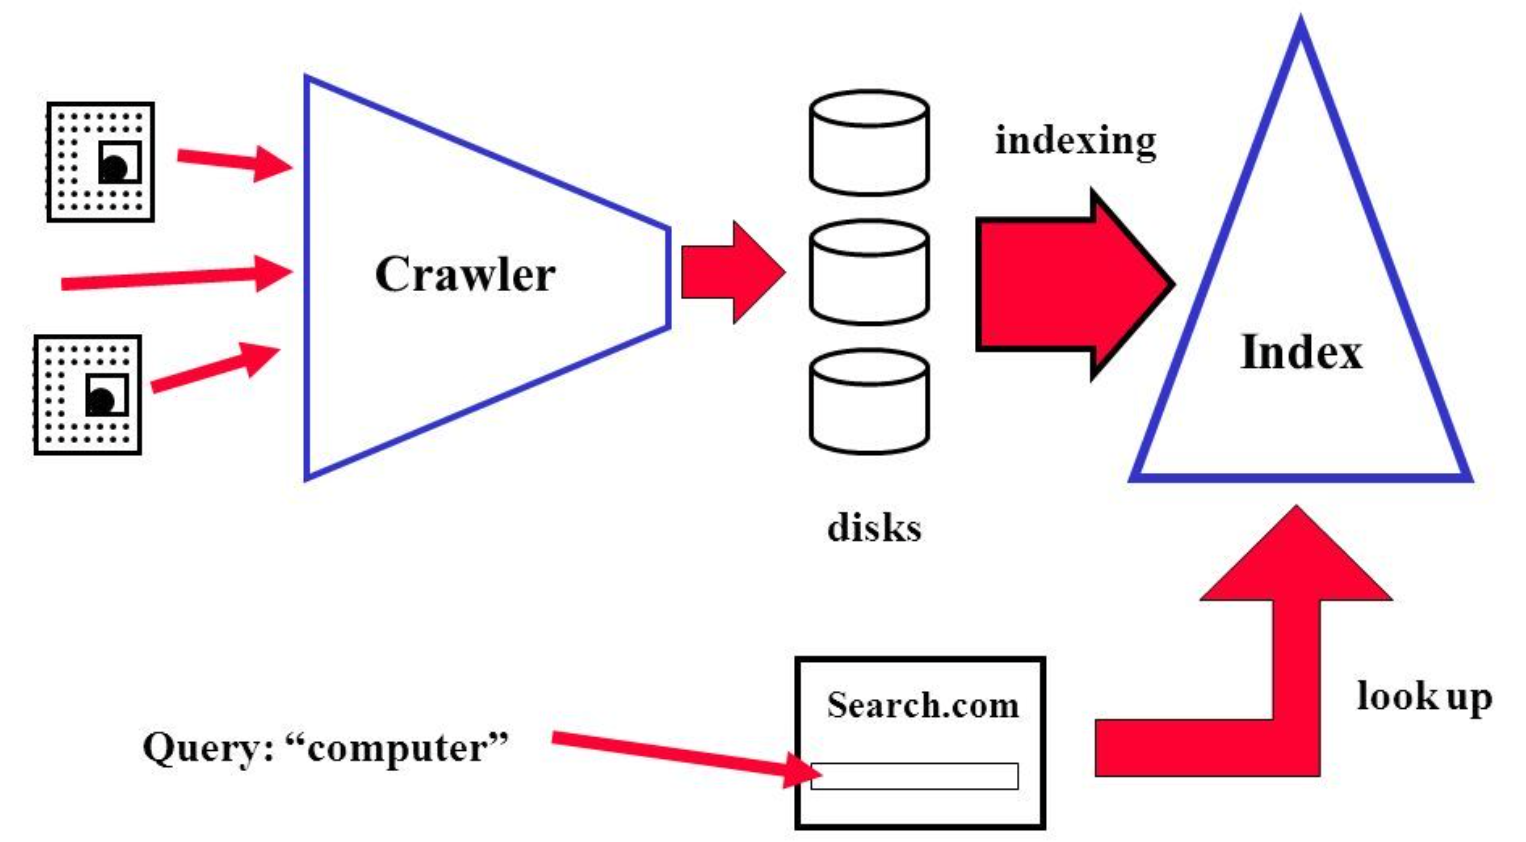
\includegraphics[width=0.8\textwidth]{assets/Search.png}
\end{center}
\end{figure}

\begin{itemize}
  \item Crawler durchsuchen das Internet und analysieren und indexieren Webseiten, Navigation über Hyperlinks (Indexierungstiefe festlegbar), Probleme durch Schranken (Deep Web) und Aktualisierungen
  \item Indizierung: Sortierung und Hinzufügen von Keywords, linguistische Verarbeitung (breitere Suche) $\rightarrow$ hohe Datenmenge, schnelle Algorithmen nötig
  \item Suche: linguistische Verarbeitung des Suchterms, Ranking der Ergebnisse möglich, Ausgabe
\end{itemize}

\subsubsection{Suchtechnologien}

\begin{itemize}
  \item Standardsoftware (teils open source) die angepasst werden kann
  \item Indexierung, Suche, \textbf{Visualisierung}: Viele Möglichkeiten, Daten aufzubereiten
  \item Open Search
  \item Kann verwendet werden um z.B. Unternehmensdaten zu durchsuchen und aufzubereiten
\end{itemize}


\subsubsection{Einsatzgebiete in der öffentlichen Verwaltung}

\begin{itemize}
  \item Struktur der Webseite ähnlich der Verwaltungsstruktur $\rightarrow$ für Bürger schwer zu durchschauen
  \item Suchmaschine als Abkürzung um zu Formular X zu kommen
  \item erleichtert Einstieg, kann Sprachbarrieren abbauen (Umgangssprache, Synonyme, Übersetzer)
  \item bei bald 575 digital zu erledigenden Verwaltungsdienstleistungen kaum ohne Suchmaschine möglich sich zum Ziel zu klicken
\end{itemize}